\documentclass[a4paper,10pt,uplatex]{jsarticle}


% 数式
\usepackage{amsmath,amssymb,amsthm,bm}
\usepackage{mathtools}
\mathtoolsset{showonlyrefs}
\usepackage{physics}
\usepackage{siunitx}
\usepackage[thicklines]{cancel}
\usepackage{comment}
\usepackage{graphicx}
\usepackage[dvipdfmx]{color}
\usepackage{here}
\usepackage{tikz}

% dvipdfmxは日本語のときのみかく
\usepackage[dvipdfmx]{hyperref}
\usepackage{pxjahyper} % (u)pLaTeXのときのみかく
\hypersetup{%
 setpagesize=false,%
 bookmarks=true,%
 bookmarksdepth=tocdepth,%
 bookmarksnumbered=true,%
 colorlinks=false,%
 pdftitle={},%
 pdfsubject={},%
 pdfauthor={},%
 pdfkeywords={}}

\numberwithin{equation}{section}

\newtheoremstyle{mystyle}%
    {3pt}%
    {3pt}%
    {}%
    {}%
    {\bfseries}%
    {:}%
    { }%
    {}%
\theoremstyle{mystyle}
\newtheorem{dfn}{定義}[section]
\newtheorem{thm}{定理}[section]
\newtheorem{lem}[thm]{補題}
\renewcommand{\proofname}{\textbf{証明}}

\newcommand{\gA}{\mathfrak{A}}
\newcommand{\gB}{\mathfrak{B}}
\newcommand{\gI}{\mathfrak{I}}
\newcommand{\gM}{\mathfrak{M}}
\newcommand{\gO}{\mathfrak{O}}
\newcommand{\gP}{\mathfrak{P}}
\newcommand{\gS}{\mathfrak{S}}

\newcommand{\R}{\mathbb{R}}

% 数式の上下のスペースの変更
\AtBeginDocument{
  \abovedisplayskip     =0.5\abovedisplayskip
  \abovedisplayshortskip=0.5\abovedisplayshortskip
  \belowdisplayskip     =0.5\belowdisplayskip
  \belowdisplayshortskip=0.5\belowdisplayshortskip
}

\begin{document}

\title{松坂「集合・位相入門」}
\author{}
\date{\today}
\maketitle

\section{位相空間}
\subsection{位相空間}
\subsubsection{位相}
\begin{dfn}[位相]
    $S$を1つの空でない集合とする.$S$の部分集合系(すなわち$\gP(S)$の部分集合)$\gO$が次の3つの条件を満たすとき,$\gO$は$S$の1つの位相構造を定める,あるいは簡単に,$\gO$は$S$における1つの位相であるという.
    \begin{enumerate}
        \item $S\in\gO$および$\phi\in\gO$. \label{dfn:位相の条件1}
        \item $O_1\in\gO$,$O_2\in\gO$ならば$O_1\cap O_2\in\gO$. \label{dfn:位相の条件2}
        \item $(O_\lambda)_{\lambda\in\Lambda}$を$\gO$の元から成る任意の集合族(すなわち,添数集合$\Lambda$は任意の有限または無限集合で,すべての$\lambda\in\Lambda$に対して$O_\lambda\in\gO$)とすれば,$\bigcup_{\lambda\in\Lambda} O_\lambda \in \gO$. \label{dfn:位相の条件3}
    \end{enumerate}
\end{dfn}

1つの位相構造の定められた集合$(S,\gO)$を位相空間という.

\subsubsection{開集合,開核}
\begin{dfn}[開集合]
    $(S,\gO)$を1つの位相空間とするとき,$\gO$に属する$S$の部分集合をこの位相空間の開集合という.
\end{dfn}
位相$\gO$はまた位相空間の開集合系ともよばれる.

\begin{dfn}[開核]
    $(S,\gO)$を1つの位相空間とし,$M\in \gP(S)$をその任意の部分集合とする.そのとき,$M$に含まれるような開集合全体の和集合$M^\circ$を$M$の開核または内部という.$M^i$とも書かれる.
\end{dfn}
$M^\circ$は$M$に含まれる最大の開集合となっている.

\begin{dfn}[開核作用子]
    $S$の各部分集合$M$にその開核$M^\circ$を対応させる写像($\gP(S)\to\gP(S)$)を開核作用子という.
\end{dfn}

\begin{thm}[開核作用子の性質]
    開核作用子は次の性質をもつ.
    \begin{enumerate}
        \item $S^\circ = S$.
        \item 任意の$M\in\gP(S)$に対して$M^\circ \subset M$.
        \item 任意の$M,N \in \gP(S)$に対して$(M \cap N)^\circ = M^\circ \cap N^\circ$.
        \item 任意の$M \in \gP(S)$に対して$M^{\circ\circ} = M^\circ$.
    \end{enumerate}
\end{thm}

\begin{thm}[開核作用子による位相構造の決定]
    逆に,上の条件を満たすような$\gP(S)$から$\gP(S)$への任意の写像は,$S$を台とするある位相空間$(S,\gO)$の開核作用子となる.この位相$\gO$は一意的に定まる.
\end{thm}

\subsubsection{閉集合,閉包}
\begin{dfn}[閉集合]
    位相空間$(S,\gO)$において,開集合の補集合として表される$S$の部分集合を,この位相空間の閉集合という.すなわち,$A\in\gP(S)$が$(S,\gO)$の閉集合であるとは,$A^c=S-A$が$\gO$の元となっていることである.
\end{dfn}

\begin{dfn}[閉包]
    $M$を位相空間$(S,\gO)$の任意の部分集合とするとき,$M$を含むような閉集合全体の共通部分$\bar{M}$を$M$の閉包という.$M^a$とも書かれる.
\end{dfn}
$\bar{M}$は$M$の最小の閉集合となっている.

\begin{thm}[閉包と開核の関係]
    \begin{equation}
        \overline{M^c} = (M^\circ)^c
    \end{equation}
    この関係は次のようにも書かれる.
    \begin{equation}
        M^{ca} = M^{ic}
    \end{equation}
    また,次の公式が導かれる.
    \begin{equation}
        M^{ca} = M^{ic}, \quad M^{cac} = M^i, \quad M^{ci} = M^{ac}, \quad M^{cic} = M^a
    \end{equation}
\end{thm}

開集合で成り立つ性質などを正反対にしたものが双対的に閉集合でも成り立つ.

\subsubsection{内点,触点,外点,境界点,集積点,孤立点}
\begin{dfn}[内点]
    $M$を位相空間$(S,\gO)$の1つの部分集合とする(以下同様).$M$の内部$M^\circ(=M^i)$に属する点を$M$の内点という.
\end{dfn}

\begin{dfn}[触点]
    $M$の閉包$\bar{M}(=M^a)$に属する点を$M$の触点という.
\end{dfn}

\begin{dfn}[外部,外点]
    $M$の補集合の内部$M^e = M^{ci}$を$M$の外部といい,$M$の外部に属する点を$M$の外点という.
\end{dfn}

\begin{dfn}[境界,境界点]
    $M$の閉包と$M$の内部との差$M^f = M^a-M^i$を$M$の境界といい,$M$の境界に属する点を$M$の境界点という.
\end{dfn}

直観的なイメージとしては,$M$は境界$M^f$がぼんやりとしているもので,$M$の内部$M^i$は境界を完全に含まない部分,閉包$M^a$は境界を完全に含む部分であり,両者の間には$M^a = M^f \cup M^i(直和)$という関係がある.包含関係は$M^i \subset M \subset M^a$である.$M$の外部は完全に$M$に属していないところで,これらを合わせると$S = M^i \cup M^f \cup M^e = M^a \cup M^e(直和)$となる.

\begin{dfn}[集積点]
    $S$の点$x$が$M-\{x\}$の触点であるとき,すなわち
    \begin{equation}
        x \in \overline{M-\{x\}}
    \end{equation}
    となるとき,$x$は$M$の集積点であるという.
\end{dfn}

\begin{dfn}[孤立点]
    $x$が$M$に属する点であって,しかも$x$が$M$の集積点でないときには,$x$は$M$の孤立点であるといわれる.
\end{dfn}

$x \notin M$のときは$M-\{x\} = M$となるから,$x$が集積点であることと$x$が触点であることとは同等となる.$x \notin M^i$だから,$x \in M^f$である.

$x \in M$のときを考える.$x$のまわりに他の$M$の要素があるなら,$M-\{x\}$は$x$の部分に点として境界があり,$(M-\{x\})^a$は$M^a$と変わりなくなる.この場合$x$は集積点である.
$x$のまわりに他の$M$の要素がない場合,つまり$x$を除くとそこが$M$の外部となってしまう場合,$x$は他の要素と孤立している,つまり孤立点である.

\subsubsection{近傍}
\begin{dfn}[近傍,近傍系]
    $(S,\gO)$を1つの位相空間とする.$x$を$S$の1つの点とするとき,$S$の部分集合$V$が$x$の近傍であるとは,$x$が$V$の内点であること,すなわち
    \begin{equation}
        x \in V^\circ
    \end{equation}
    が成り立つことをいう.また,$x$の近傍の全体を$x$の(全)近傍系とよぶ.以下これを$\bm{V}(x)$で表す.
\end{dfn}

\begin{thm}[開集合の近傍による特徴づけ]
    $S$の空でない部分集合$O$が開集合であるための必要十分条件は,$O$の任意の点$x$に対して,$O$が$x$の近傍となっていることである.
\end{thm}

\begin{thm}[近傍系の性質]
    位相空間$(S,\gO)$の各点$x$の近傍系$\bm{V}(x)$について次のことが成り立つ.
    \begin{enumerate}
        \item すべての$V\in\bm{V}(x)$に対して,$x\in V$.
        \item $V\in\bm{V}(x)$で$V\subset V' (V' \in \gP(S))$ならば,$V' \in \bm{V}(x)$.
        \item $V_1 \in \bm{V}(x), V_2 \in \bm{V}(x)$ならば,$V_1\cap V_2 \in \bm{V}(x)$.
        \item 任意の$V \in \bm{V}(x)$に対して,次の条件を満たす$W \in \bm{V}(x)$が存在する:$W$の任意の点$y$に対して$V \in \bm{V}(y)$.
    \end{enumerate}
\end{thm}

\begin{thm}[近傍系による位相構造の決定]
    空でない集合$S$の各点$x$に対しそれぞれ1つずつ$\gP(S)$の空でない部分集合$\bm{V}(x)$が定められ,上の条件1〜4が成り立つとする.そのとき,$S$に1つの位相$\gO$を導入して,与えられた$\bm{V}(x)$が位相空間$(S,\gO)$における$x$の近傍系となるようにすることができる.かつ,そのような$\gO$は一意的に定まる.
\end{thm}

\subsubsection{まとめ}
集合$S$に位相構造を定めるには,
\begin{itemize}
    \item 開集合系
    \item 閉集合系
    \item 開核作用子
    \item 閉包作用子
    \item 近傍系
\end{itemize}
のいずれか1つを与えればよく,これらのうちの1つを与えれば,ほかはそれから必然的にそれぞれ一意的に定まる.

\subsection{位相の比較,位相の生成}
\subsubsection{位相の強弱}
\begin{dfn}[位相の強弱]
    $\gO_1, \gO_2$が$S$における2つの位相であって,
    \begin{equation}
        \gO_1 \subset \gO_2
    \end{equation}
    が成り立つとき,位相$\gO_1$は位相$\gO_2$よりも弱い,$\gO_2$は$\gO_1$よりも強いという.(このことを$\gO_1 \leq \gO_2$と書くこともある.)
\end{dfn}

\begin{thm}[位相の強弱と同等な条件]
    $S$における2つの位相$\gO_1, \gO_2$から定まる閉集合系をそれぞれ$\gA_1,\gA_2$;近傍系をそれぞれ$\bm{V}_1(x), \bm{V}_2(x)$とすれば,$\gO_1$が$\gO_2$よりも弱いことは,次の条件1あるいは2と同等である.
    \begin{enumerate}
        \item $\gA_1 \subset \gA_2$
        \item $S$の任意の点$x$に対して$\bm{V}_1(x) \subset \bm{V}_2(x)$
    \end{enumerate}
\end{thm}

\begin{dfn}[完備束] 
    順序集合$M$において,その任意の空でない部分集合が($M$の中に)上限および下限を有するとき,$M$は完備束であるといわれる.
\end{dfn}

\begin{thm}[位相の強弱による順序集合] \label{thm:位相の強弱による順序集合}
    $S$を1つの空でない集合とするとき,$S$において定義される位相全体の集合$\gI(S)=\gI$は,強弱の順序について完備束をなす.$(\gO_\alpha)_{\alpha\in A}$を$\gI$の元からなる任意の族とするとき,$\inf\{\gO_\alpha | \alpha \in A\}$は共通部分$\bigcap_{\alpha \in A}\gO_\alpha$である.また$\sup\{\gO_\alpha | \alpha \in A\}$は,和集合$\bigcup_{\alpha \in A}\gO_\alpha$を含むような$\gI$の元全体の共通部分である.
\end{thm}

\subsubsection{位相の生成}
\begin{dfn}[位相の生成]
    $S$を空でない1つの集合とする.$\gP(S)$の任意の部分集合$\gM$について,$\gM$を含むような$S$における位相全部の集合の下限を$\gO(\gM)$とする(定理\ref{thm:位相の強弱による順序集合}より存在は保証される).$\gO(\gM)$を,$\gM$で生成される位相という.
\end{dfn}

\begin{thm}[生成される位相の内容]
    $\gM$を$\gP(S)$の任意の部分集合とするとき,$\gM$で生成される$S$における位相$\gO(\gM)$は,$\bigcup_{\lambda \in \Lambda}B_\lambda (B_\lambda \in \gM_0,\Lambda の濃度は任意)$の形に表される集合の全体から成る($\Lambda = \phi$のときは$\phi$を意味するものとする).ただし,ここで$\gM_0$は$\bigcap_{i \in I} A_i (A_i \in \gM,Iは有限集合)$の形に表される集合の全体である($I = \phi$のときは$S$を意味するものとする).
\end{thm}

$\gM_0 = \bigcap_{i \in I} A_i (A_i \in \gM,Iは有限集合)$は,$I$のサイズが0のとき$S$,1のとき$\gM$,2以上のとき$\gM$の元の共通部分であるから,包含関係は$\gM \subset \gM_0$となっている.$\gM$だけでは位相の条件(開集合系の条件)の\ref{dfn:位相の条件1}と\ref{dfn:位相の条件2}を満たしているとは限らないため,不足分を付け足した$\gM_0$をまず作るのだ.$\gM_0$は条件\ref{dfn:位相の条件1}と\ref{dfn:位相の条件2}を満たしている.最後に条件\ref{dfn:位相の条件3}を満たすために,全体の和集合をとる.これによって位相$\gO$が出来上がる.包含関係は$\gM \subset \gM_0 \subset \gO$.

\subsubsection{位相の準基底,基底}
\begin{dfn}[準基底]
    $S$における1つの位相$\gO$が与えられたとき,$\gO$のある部分集合$\gM$に対して$\gO = \gO(\gM)$が成り立つならば,$\gM$は位相$\gO$の準基底であるという.
\end{dfn}
$\gO$に対してその準基底は一意的には定まらない.

\begin{dfn}[基底]
    $\gB$が位相$\gO$の部分集合で,$\gO$の任意の元$O$は,$O$に含まれる$\gB$の元の和集合として
    \begin{equation}
        O = \bigcup_{\lambda \in \Lambda} W_\lambda, \quad W_\lambda \in \gB, \Lambda の濃度は任意
    \end{equation}
    と表されるとき,$\gB$は$\gO$の基底であるという.
\end{dfn}
$\gO$に対してその基底は一意的には定まらない.

\begin{figure}[h]
    \begin{center}
    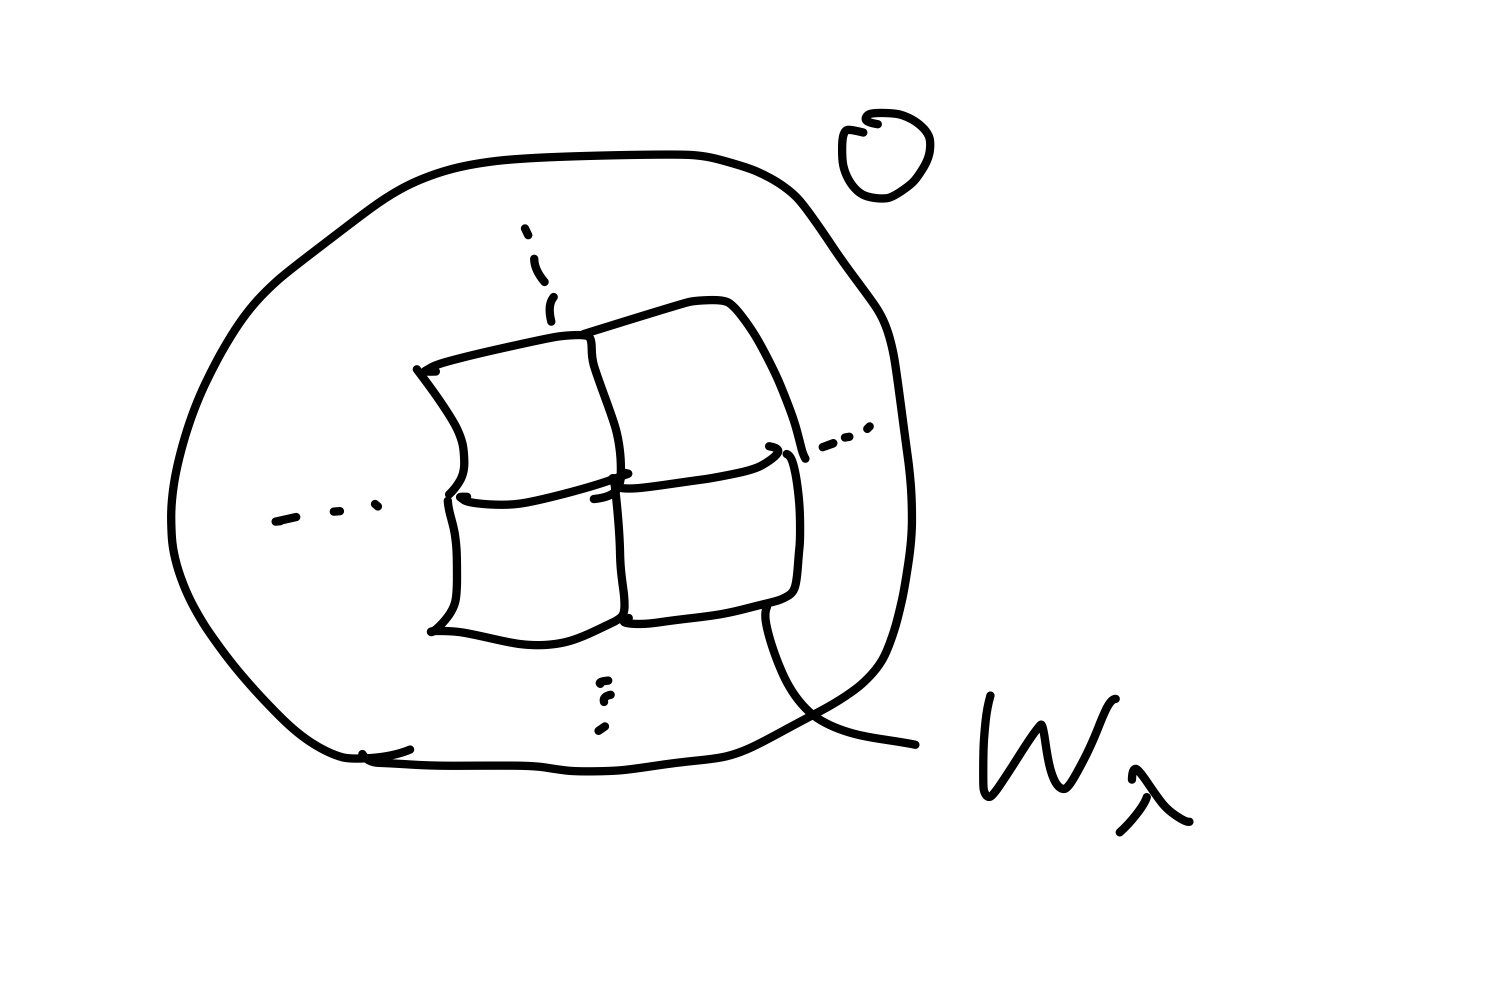
\includegraphics[width = 50mm]{基底.jpeg}
    \caption{基底の定義のイメージ図}
    \end{center}
\end{figure}

$\gB$が$\gO$の基底であるということは$\gB$には$\gO$を構成する最低限のパーツ(開集合)は揃っているということで,上の定義は$\gB$の元を適当に貼り合わせれば$\gO$の任意の元が作り出せることを表している.
基底ではないが準基底であるものは,大きいパーツしかなくて$\gO$の小さな元が表せないが,交わりをとって小さな元を補うことで最低限のパーツが揃う.
基底が位相の"もと"であるとしたら,準基底は基底の"もと"だとも言えそうだ.

\begin{thm}[基底であることの条件]
    $\gO$を$S$における1つの位相とするとき,その部分集合$\gB$が$\gO$の基底となるためには,任意の$O\in\gO$および任意の$x\in O$に対して,
    \begin{equation}
        x \in W, \quad W \subset O
    \end{equation}
    となるような$W \in \gB$が存在することが必要十分である.
\end{thm}

\begin{dfn}[第2可算公理]
    位相空間$(S,\gO)$において,たかだか可算の基底$\gB$(すなわち$\mathrm{card}\gB \leq \aleph_0$であるような$\gO$の基底$\gB$)が存在するとき,$(S,\gO)$は第2可算公理を満足するという.
\end{dfn}

例えば$\mathbb{R}^n$に位相として開球体
\begin{equation}
    B(x;\varepsilon) \quad (x \in \mathbb{R}^n, \varepsilon > 0)
\end{equation}
全体の集合系を入れた位相空間を考えると,基底として有理数半径の開球体全体の集合系をとれる.これは可算だから,位相空間$\mathbb{R}^n$は第2可算公理を満足する.

\subsubsection{基本近傍系}
\begin{dfn}[基本近傍系]
    $(S,\gO)$を1つの位相空間とし,$\bm{V}(x)$を点$x$の近傍系とする.$\bm{V}(x)$の部分集合$\bm{V}^*(x)$で次の性質をもつものを,$x$の基本近傍系という.
    \begin{itemize}
        \item[] 任意の$V \in \bm{V}(x)$に対して,$U \subset V$となるような$U \in \bm{V}^*(x)$が存在する.
    \end{itemize}
\end{dfn}
例えば$x$を含む開集合全体の集まり$\bm{V}_\gO^*(x)$や,基底$\gB$の$x$を含む元全体の集合$\bm{V}_\gB^*(x)$が基本近傍系としてとれる.
基本近傍系は,(全)近傍系の"もと"になるようなものである.実際,
\begin{equation}
    \bm{V}(x) = \{V | \exists U \in \bm{V}^*(x) (U \subset V)\}
\end{equation}
と,基本近傍系から(全)近傍系を構成できる.

\begin{dfn}[第1可算公理]
    位相空間$(S,\gO)$において,$S$の各点$x$がたかだか可算の基本近傍系$\bm{V}^*(x)$をもつとき,$(S,\gO)$は第1可算公理を満足するという.
\end{dfn}

\begin{thm}
    位相空間$(S,\gO)$が第2可算公理を満足すれば,第1可算公理も満足する.
\end{thm}
例えば$\bm{V}_\gB^*(x)$は基底$\gB$と$\bm{V}_\gB^*(x) \subset \gB$という関係にあるので,第2可算公理を満足していれば当然第1可算公理も満足する.

\subsubsection{可分位相空間}
\begin{dfn}[密,稠密]
    位相空間$(S,\gO)$の部分集合$M$について,$\bar{M} = S$が成り立つとき,$M$は$S$において密または稠密であるという.
\end{dfn}
$M^a = S \Leftrightarrow M^{ci} = M^e = \phi$より,$M$が$S$において密であることは$M$の外部に開集合が存在しないことを表している.

$(S,\gO)$の1つの基底$\gB$が与えられたとする.基底は$S$をいくつかの部品(開集合)に分解したものの集合であり,位相$\gO$の"もと"となるものである.基底の各元$B \in \gB$から1つの元$x_B \in B$をとって$S$の部分集合$M = \{x_B | B \in \gB\}$を作ると,$M^c$は,どの基底の元にとっても少なくとも1つ穴が開いているようになる.つまり,$M$の外部には開集合が存在しない.したがってこの部分集合$M$は$S$において密である.

\begin{dfn}[可分]
    位相空間$(S,\gO)$のたかだか可算なある部分集合が$S$において密となるとき,$(S,\gO)$は可分な位相空間であるといわれる
\end{dfn}

先に挙げた例を見ると,部分集合$M$が基底のすべての元の要素を含むくらい満遍ないとき,$M$は$S$において密である,と言える.だから,可分な位相空間の条件,可算なある部分集合が$S$において密となるということは,基底のすべての元の要素が可算個であるということになる.
そもそも基底が可算であれば,必ず可分になるため,以下の定理が従う.

\begin{thm}
    第2可算公理を満足する任意の位相空間は可分である.
\end{thm}

逆は成立しない.部分集合$M$の1個の要素が,非加算個の基底の元の共通部分に属する場合などが考えられる.

\subsection{連続写像}
\subsubsection{連続写像}
$(S,\gO)$、$(S',\gO')$を2つの位相空間とする.以下,これらを単に$S,S'$と略記する.

\begin{thm}[連続写像の条件]
    $f$を$S$から$S'$への与えられた1つの写像とする.位相空間$S,S'$の閉集合系をそれぞれ$\gA,\gA'$とし,$S,S'$の点$x,x'$の($S,S'$における)近傍系を$\bm{V}_S(x), \bm{V}_{S'}(x')$とする.そのとき,($f$に関する)次の3条件は互いに同等である.
    \begin{enumerate}
        \item \hfill
        \vspace{-\abovedisplayskip} 
        \begin{equation}
            O' \in \gO' \Rightarrow f^{-1}(O') \in \gO.
        \end{equation} \label{thm:連続写像の条件1}
        \item \hfill
        \vspace{-\abovedisplayskip}
        \begin{equation}
            A' \in \gA' \Rightarrow f^{-1}(A') \in \gA.
        \end{equation}
        \item $S$の各点$x$に対し,$f(x) = x'$とすれば
        %\vspace{-\abovedisplayskip}
        \begin{equation}
            V' \in \bm{V}_{S'}(x') \Rightarrow f^{-1}(V') \in \bm{V}_S(x).
        \end{equation} \label{thm:連続写像の条件3}
    \end{enumerate}
\end{thm}

\begin{dfn}[連続写像]
    上の3つの条件のうちいずれか(したがって全部)が成り立つとき,$f$は$S$から$S'$への連続写像であるという.
\end{dfn}

\begin{thm}[準基底による連続写像の条件] \label{thm:準基底による連続写像の条件}
    写像$f:S \to S'$が連続であるためには,$\gM'$を位相空間$S'$の1つの準基底(すなわち$\gO(\gM') = \gO'$)とするとき,任意の$M \in \gM'$に対して$f^{-1}(M) \in \gO$となることが,必要かつ十分である.
\end{thm}
これは連続写像の条件\ref{thm:連続写像の条件1}を弱めたもの.定理の条件を論理式で書くとわかりやすい:
\begin{equation}
    M \in \gM' \Rightarrow f^{-1}(M) \in \gO
\end{equation}
$\gM' \subset \gO'$だから$M \in \gO'$で,必要であることは明らか.十分性を示すためには次の補題を使う(こちらの方が本質的に重要な気がする).

\begin{lem}
    集合系$\gS$を,$f^{-1}(M) \in \gO$となるような$S'$の部分集合$M$全体からなるものとする.つまり,
    \begin{equation}
        \gS = \{M | f^{-1}(M) \in \gO\}
    \end{equation}
    とする.このとき,$\gS$は$S'$における位相である.
\end{lem}
これを認めれば,$\gM' \subset \gS$より$\gO' \subset \gS$.したがって$O' \in \gO'$は$O' \in \gS$でもあり,$f^{-1}(O') \in \gO$を満たす.つまり\ref{thm:連続写像の条件1}が満たされる.$\gO' \subset \gS$というのが肝である.こうなるような条件のうち,最も緩いのが準基底を使ったものなのだ($準基底 \subset 基底 \subset 位相$だから).

\begin{dfn}[連続]
    $f$が$S$から$S'$への写像で,連続写像の条件\ref{thm:連続写像の条件3}が$S$の全ての点の代わりに$S$のある1点$x_0$に対して成り立つとき,すなわち
    \begin{equation}
        V' \in \bm{V}_{S'}(x_0') \Rightarrow f^{-1}(V') \in \bm{V}_S(x_0)
    \end{equation}
    が成立するとき,$f$は点$x_0$において連続であるという.
\end{dfn}

\begin{thm}[基本近傍系による連続の条件] \label{thm:基本近傍系による連続の条件}
    上記の連続の条件は,基本近傍系$\bm{V}_{S'}^*(x_0')$によって
    \begin{equation}
        V'^* \in \bm{V}_{S'}^*(x_0') \Rightarrow f^{-1}(V') \in \bm{V}_S(x_0)
    \end{equation}
    と置き換えても同じことになる.
\end{thm}

\begin{proof}
    必要性は$\bm{V}_{S'}^*(x_0') \subset \bm{V}_{S'}(x_0')$より明らか.十分性を示す.$V' \in \bm{V}_{S'}(x_0')$とする.このとき$V'^* \subset V'$なる$V'^* \in \bm{V}_{S'}^*(x_0')$が存在する.よって
    \begin{equation}
        f^{-1}(V'^*) \subset f^{-1}(V')
    \end{equation}
    仮定より$f^{-1}(V'^*) \in \bm{V}_{S}(x_0)$だから,$f^{-1}(V') \in \bm{V}_{S}(x_0)$.
\end{proof}
$\bm{V}_{S'}(x_0') \subset \bm{V}_{S'}^*(x_0')$だから直感的にはわかりづらいが,近傍は$A \subset B$で$A \in \bm{V}(x)$ならば$B \in \bm{V}(x)$という性質に注意すればわかる.

\subsubsection{実連続関数}
\begin{dfn}[実数値関数,実連続関数]
    位相空間$S$から実数全体の集合が作る位相空間$\R$への一般の写像を$S$上の実数値関数とよび,そのうち$S$から$\R$への連続写像であるものを実連続関数という.
\end{dfn}

\begin{thm}[実連続関数であるための条件]
    位相空間$S$で定義された実数値関数$f$が実連続関数であるためには,次の1,2,3のいずれかが成り立つことが必要十分である.
    \begin{enumerate}
        \item $\R$の任意の開区間$(a,b)$に対して
        \begin{equation}
            f^{-1}((a,b)) = \{x | x \in S, a<f(x)<b\}
        \end{equation}
        は$S$の開集合である.

        \item 任意の実数$a,b$に対して
        \begin{equation}
            f^{-1}((a,\infty)) = \{x | x \in S, f(x) > a\}
        \end{equation}
        および
        \begin{equation}
            f^{-1}((-\infty,b)) = \{x | x \in S, f(x) < b\}
        \end{equation}
        は$S$の開集合である.

        \item $x_0$を$S$の任意の点とするとき,任意の正の実数$\varepsilon$に対して
        \begin{align}
            &f^{-1}((f(x_0)-\varepsilon, f(x_0)+\varepsilon)) \\
            &\quad = \{x \in S, |f(x) - f(x_0)| < \varepsilon\}
        \end{align}
        は$x_0$の$S$における近傍である.
    \end{enumerate}
\end{thm}
これらは,$\R$の任意の開集合が$(a,b)$で表されること,準基底として$(a,\infty)$および$(-\infty,b)$の形の区間全体がとれること,$x_0$の基本近傍系として$(x_0 - \varepsilon, x_0 + \varepsilon)$の形の区間全体をとることができることを,それぞれ,連続写像の条件\ref{thm:連続写像の条件1},準基底による連続写像の条件\ref{thm:準基底による連続写像の条件},基本近傍系による連続の条件\ref{thm:基本近傍系による連続の条件}に適用したもの.

\begin{thm}[連続関数の和,差,積,商]
    $f,g$がともに位相空間$S$で定義された実連続関数ならば,$f+g, f-g, f\cdot g, af(a\in\R)$も実連続関数である.また,$S$のすべての点$x$において$g(x)\neq 0$ならば,$f/g$も実連続関数である.
\end{thm} 

\end{document}
